\section{Vida \'util de estruturas de concreto armado}\label{sec:vida_util}

% SECAO NOVA: reune a fundamentacao sobre degradacao, carbonatacao, modelo de
% previsao e vida util remanescente. Os blocos de fenomenologia e do modelo de
% Possan foram transferidos da antiga Secao de Metodologia; a Metodologia passa a
% conter apenas o que foi efetivamente decidido e executado neste trabalho.

\subsection{Degrada\c{c}\~ao, vida \'util e o modelo de Tuutti}
\label{subsec:degradacao}

Estruturas de concreto armado em serviço estão permanentemente expostas a agentes físicos e químicos que reduzem progressivamente seu desempenho. A durabilidade não é, portanto, uma propriedade intrínseca do material, mas a resposta de uma estrutura específica, em um ambiente específico, ao longo de um período determinado \parencite{fib2006}. Essa dependência conjunta de material, ambiente e tempo é o que torna a previsão de vida útil um problema naturalmente probabilístico.

Entre os mecanismos de deterioração do concreto armado destacam-se a corrosão de armaduras induzida por íons cloreto, característica de ambientes marinhos e de estruturas sujeitas a sais de degelo; a corrosão induzida por carbonatação, predominante em ambientes urbanos e atmosféricos; o ataque por sulfatos; a reação álcali-agregado; a lixiviação da matriz cimentícia; e os ciclos de gelo-degelo. Dentre todos, a corrosão das armaduras é reconhecida como a principal causa de deterioração precoce de estruturas de concreto armado \parencite{tuutti1982, melchers2018}.

Os dois mecanismos de corrosão mais relevantes diferem quanto à natureza do ataque, conforme detalhado na Seção~\ref{subsub:fenomenologia}: os cloretos rompem a camada passiva de forma localizada, enquanto a carbonatação a destrói de maneira generalizada. A carbonatação é o mecanismo dominante em ambientes urbanos atmosféricos afastados da orla marítima, condição que descreve grande parte do parque construído brasileiro no interior do país e que justifica o recorte adotado neste trabalho.

No que se refere à vida útil, é usual distinguir a \textit{vida útil de projeto}, período para o qual a estrutura é concebida e que fundamenta a escolha do cobrimento e da classe de agressividade ambiental \parencite{nbr6118}; a \textit{vida útil de serviço}, efetivamente observada em campo; e a \textit{vida útil remanescente}, isto é, o período que resta, a partir de um instante de inspeção, até que um estado limite pertinente seja atingido. É esta última que interessa à gestão de ativos existentes e que constitui o objeto deste trabalho.

O arcabouço conceitual consagrado para descrever a evolução da corrosão é o modelo de \textcite{tuutti1982}, que decompõe a vida útil em duas fases sucessivas:

\begin{equation}\label{eq:tuutti}
t_{\mathrm{total}} = t_{\mathrm{ini}} + t_{\mathrm{prop}},
\end{equation}

\noindent em que $t_{\mathrm{ini}}$ é o período de \textit{iniciação}, durante o qual a frente agressiva avança pelo cobrimento sem que haja perda de capacidade estrutural, e $t_{\mathrm{prop}}$ é o período de \textit{propagação}, iniciado com a despassivação da armadura, no qual ocorrem a perda de seção do aço, a fissuração por expansão dos produtos de corrosão e o eventual destacamento do cobrimento.

Este trabalho concentra-se na \textbf{fase de iniciação}. O estado limite considerado é, portanto, a \textit{despassivação} da armadura --- o instante em que a frente carbonatada alcança o nível do aço --- e não a ruína estrutural. Trata-se de um estado limite de serviço de durabilidade, para o qual as recomendações do \textcite{fib2006} indicam índices de confiabilidade alvo da ordem de $\beta_{\mathrm{alvo}} \approx 1{,}3$, substancialmente inferiores aos adotados para estados limites últimos, justamente porque sua violação não implica colapso, mas o encerramento do período protegido e o início da janela em que a intervenção de manutenção passa a ser pertinente. Essa distinção é mantida explicitamente ao longo de todo o texto: as distribuições de vida útil remanescente aqui obtidas referem-se ao tempo até a despassivação.

\subsection{Carbonata\c{c}\~ao: fenomenologia}
\label{subsub:fenomenologia}

A corrosão desencadeada pela carbonatação difere substancialmente de outros mecanismos agressivos por sua natureza química global, governada pela redução progressiva da alcalinidade da matriz cimentícia. Enquanto agentes como os íons cloreto perfuram a camada passiva de forma localizada (corrosão por \textit{pites}), a carbonatação avança como uma frente ácida que reduz o pH do concreto a níveis inferiores a 9, promovendo a despassivação generalizada de toda a superfície da armadura afetada. Essa perda de proteção em larga escala resulta em corrosão uniforme, caracterizada pela formação volumosa de óxidos expansivos ao longo da barra, o que gera tensões de tração no concreto e culmina em fissuração intensa e destacamento do cobrimento, mesmo antes da perda crítica de seção transversal do aço \parencite{tuutti1982}.

O processo inicia-se com a difusão do dióxido de carbono atmosférico (CO$_2$) através da rede de poros do concreto. O CO$_2$ reage com a umidade dos poros e com os produtos de hidratação do cimento, predominantemente o hidróxido de cálcio (Ca(OH)$_2$), levando à formação de carbonato de cálcio (CaCO$_3$), conforme a Equação~\eqref{eq:carbonation}:

\begin{equation}\label{eq:carbonation}
\mathrm{Ca(OH)_2 + CO_2 \rightarrow CaCO_3 + H_2O}
\end{equation}

Em condições normais, o concreto mantém um ambiente altamente alcalino (pH entre 12,6 e 13,5), que sustenta uma película passiva estável de óxidos sobre a superfície do aço, conferindo proteção efetiva contra a corrosão. O avanço progressivo da frente de carbonatação, contudo, reduz o pH a valores inferiores a 9, despassivando a armadura e tornando o aço suscetível à corrosão generalizada na presença de oxigênio e umidade. O processo de corrosão é tipicamente dividido em duas fases: \textit{iniciação}, durante a qual a armadura permanece passivada enquanto a frente avança em direção a ela, e \textit{propagação}, na qual a película protetora é destruída e a corrosão ativa se desenvolve \parencite{tuutti1982}.

A velocidade e a profundidade da carbonatação são influenciadas por diversos fatores ambientais e de material, tais como: a concentração de CO$_2$ (níveis mais elevados aceleram a reação); a umidade relativa do ar (a carbonatação é mais intensa em faixas intermediárias, tipicamente 50\%--70\%); a qualidade do concreto (relação água/cimento, tipo de cimento e porosidade determinam a facilidade de ingresso do CO$_2$); e a espessura do cobrimento, que atua como barreira física \parencite{possan2010, possan2016co2}.

\begin{figure}[htpb!]
    \centering
    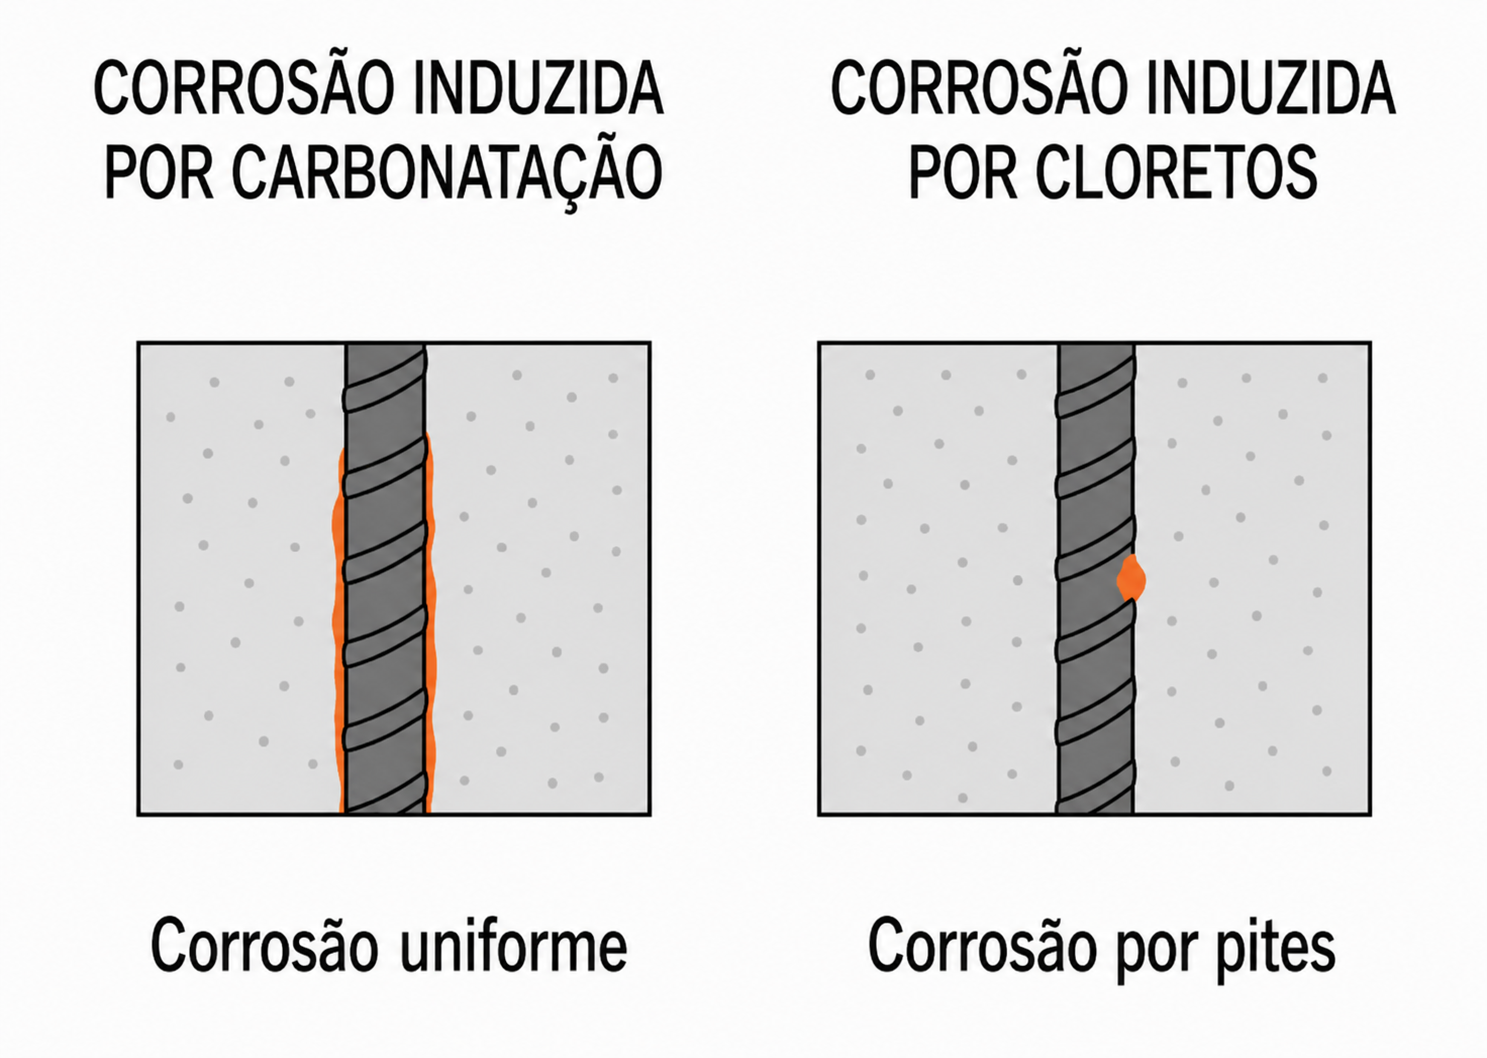
\includegraphics[width=0.5\linewidth]{z_corrosion_pt.png}
    \caption{Diferenças entre os mecanismos de corrosão localizada (cloretos) e generalizada (carbonatação).}
    \label{fig:z_corrosion_pt}
\end{figure}

\subsection{Exposi\c{c}\~ao ambiental: concentra\c{c}\~ao atmosf\'erica de \texorpdfstring{CO$_2$}{CO2}}
\label{subsec:co2_cenarios}

Como descrito na subseção anterior, o CO$_2$ atmosférico é o agente que desencadeia a carbonatação, e sua concentração governa diretamente o fluxo difusivo para o interior do concreto. Diferentemente das demais condições ambientais, trata-se de uma grandeza que não é estacionária ao longo da vida útil de uma estrutura: a concentração de fundo cresceu de forma sustentada ao longo do século XX e sua trajetória futura depende do cenário de emissões considerado. Uma previsão de vida útil em horizonte secular precisa, portanto, tratar o CO$_2$ como uma condição de exposição variável no tempo, e não como uma constante. Para representar sua evolução, empregam-se as concentrações médias globais anuais do CMIP6, publicadas por \textcite{meinshausen2017} para o período histórico e por \textcite{meinshausen2020} para os cenários SSP (\textit{Shared Socioeconomic Pathways}). A grandeza utilizada é a concentração de CO$_2$ no ar, em partes por milhão (ppm), e não a taxa de emissão, o consumo de carbono ou uma concentração de CO$_2$ equivalente.

A série implementada abrange 1900--2100. Até 2014, adota-se um histórico comum aos cenários. A partir de 2015, utilizam-se as trajetórias anuais publicadas para SSP1-2.6, SSP2-4.5 e SSP5-8.5. Os dados foram extraídos das colunas referentes a CO$_2$, unidade ppm e região global (\textit{World}) do suplemento de \textcite{meinshausen2020}; o mesmo suplemento disponibiliza a série histórica de \textcite{meinshausen2017}. As séries são utilizadas sem ajuste de regressão ou correção posterior. As abas SSP incorporam observações em 2015--2016, conforme a descrição da base, e as trajetórias subsequentes são mantidas na versão publicada em 2020. Assim, os valores de cenário em anos já transcorridos não são apresentados como medições atualizadas.

Os três cenários representam, respectivamente, trajetórias de emissões baixas, intermediárias e muito altas. Sua seleção permite examinar condições ambientais contrastantes sem atribuir probabilidades de ocorrência. O SSP2-4.5 é a referência de comparação adotada por padrão; essa escolha não implica classificá-lo como o futuro mais provável. Na nomenclatura SSP$x$-$y$, o primeiro índice identifica a trajetória socioeconômica e o segundo indica o nível aproximado de forçamento radiativo em 2100, em W/m$^2$ \parencite{ipcc2021scenarios}. Os resultados de durabilidade devem, portanto, ser interpretados como condicionais ao cenário de exposição escolhido.

\begin{figure}[htbp]
    \centering
    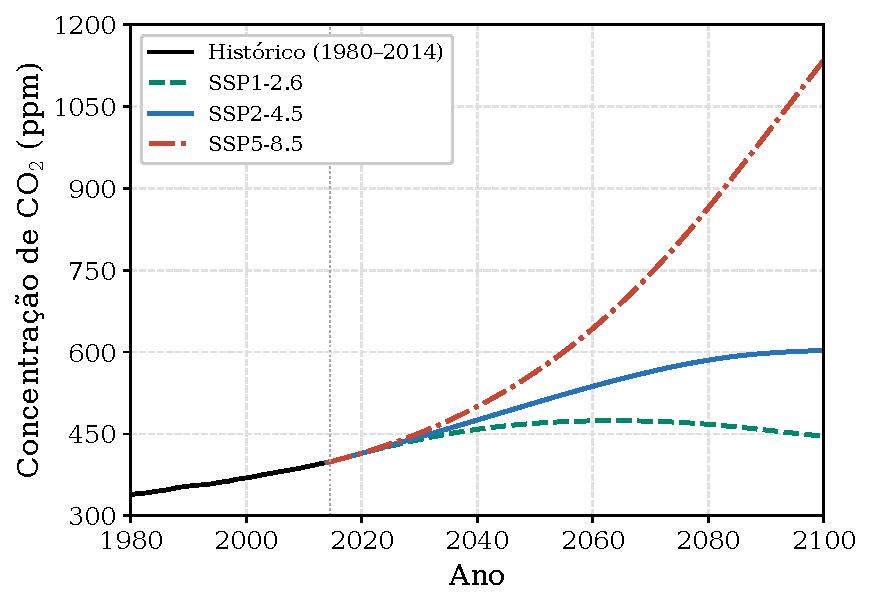
\includegraphics[width=0.82\linewidth]{z_co2_scenarios_pt.pdf}
    \caption{Concentração atmosférica média global anual de CO$_2$ entre 1980 e 2100: histórico comum até 2014 e trajetórias SSP1-2.6, SSP2-4.5 e SSP5-8.5 a partir de 2015. A linha vertical indica a transição entre as séries. As linhas unem os valores anuais publicados e não representam bandas de confiança. Elaboração própria com dados de \textcite{meinshausen2017,meinshausen2020}.}
    \label{fig:evolution_co2}
\end{figure}

A Figura~\ref{fig:evolution_co2} evidencia a divergência entre as trajetórias. No SSP1-2.6, a concentração atinge aproximadamente 474~ppm em 2063 e posteriormente diminui; no SSP2-4.5, o crescimento desacelera; no SSP5-8.5, o aumento é mais acentuado. A Tabela~\ref{tab:co2_scenarios} apresenta valores selecionados para os horizontes de interesse. Esses valores descrevem o CO$_2$ atmosférico; uma eventual redução da concentração não significa reversão da carbonatação já ocorrida.

\begin{table}[htbp]
    \centering
    \caption{Concentrações médias globais anuais de CO$_2$ nos cenários adotados (ppm), extraídas do suplemento de \textcite{meinshausen2020}.}
    \label{tab:co2_scenarios}
    \begin{tabular}{lrrr}
        \toprule
        Cenário & 2050 & 2080 & 2100 \\
        \midrule
        SSP1-2.6 & 469,3 & 467,4 & 445,6 \\
        SSP2-4.5 & 506,9 & 585,1 & 602,8 \\
        SSP5-8.5 & 562,8 & 864,4 & 1135,2 \\
        \bottomrule
    \end{tabular}
\end{table}

\subsection{Modelos de previs\~ao da profundidade de carbonata\c{c}\~ao}
\label{subsec:modelo_possan}

A despassivação por carbonatação ocorre quando a frente carbonatada avança pelo concreto de cobrimento e atinge o nível da armadura, ou seja, quando $y(t) \geq c_{\mathrm{nom}}$, sendo $c_{\mathrm{nom}}$ o cobrimento nominal. Para prever o avanço dessa frente ao longo do tempo, existem diversos modelos matemáticos na literatura, que variam desde formulações empíricas simples até abordagens analíticas e mecanísticas mais complexas.

Na sua forma mais geral e clássica, frequentemente utilizada em análises de confiabilidade, o avanço da frente de carbonatação reduz-se à lei da difusão baseada na raiz do tempo:

\begin{equation}\label{eq:raiz_t}
y(t) = k\,\sqrt{t},
\end{equation}

\noindent na qual $t$ é o tempo de exposição e $k$ (mm/$\sqrt{\text{ano}}$) é o coeficiente de carbonatação. Em modelos simplificados como este, o coeficiente $k$ condensa todo o efeito conjunto do material e do ambiente de exposição, podendo ser obtido, por exemplo, por regressão de perfis medidos como $k = y/\sqrt{t}$. A contrapartida dessa simplicidade é que $k$ não permite discriminar a contribuição individual de cada fator de projeto ou de ambiente, o que o torna pouco útil quando o objetivo é justamente propagar incertezas de material e de exposição, como neste trabalho.

\paragraph{Formula\c{c}\~ao adotada.} Para contornar essa limitação, adotou-se o modelo semiempírico de \textcite{possan2010, possan2016co2}, calibrado a partir de resultados de ensaios naturais e acelerados de concretos brasileiros. O modelo explicita a influência da resistência à compressão, do tipo de cimento, do teor de adições pozolânicas, da concentração atmosférica de CO$_2$, da umidade relativa e da proteção à chuva, conforme a Equação~\eqref{eq:y}:

\begin{equation}\label{eq:y}
y(t) = k_c \cdot \left( \frac{20}{f_c} \right)^{k_{fc}} \cdot \left( \frac{t}{20} \right)^{\frac{1}{2}} \cdot \exp \left[ \frac{k_{ad} \cdot ad^{\frac{3}{2}}}{40 + f_c} + \frac{k_{CO_2} \cdot CO_2^{\frac{1}{2}}}{60 + f_c} - \frac{k_{UR} \cdot (UR - 0{,}58)^2}{100 + f_c} \right] \cdot k_{ce}
\end{equation}

\noindent em que $y(t)$ é a profundidade de carbonatação (mm) na idade $t$ (anos), $f_c$ é a resistência à compressão do concreto (MPa), $ad$ é o teor de adição pozolânica em relação à massa de cimento (\%), $CO_2$ é a concentração volumétrica de dióxido de carbono no ambiente (\%) e $UR$ é a umidade relativa média do ar, expressa como fração decimal. Os seis coeficientes de calibração são: $k_c$, associado ao tipo de cimento; $k_{fc}$, à resistência à compressão; $k_{ad}$, às adições pozolânicas; $k_{CO_2}$, à concentração de CO$_2$; $k_{UR}$, à umidade relativa; e $k_{ce}$, à condição de exposição da estrutura quanto à proteção à chuva. Os cinco primeiros dependem do tipo de cimento e o último da condição de exposição, com os valores reunidos na Tabela~\ref{tab:coef_possan}.

\begin{table}[htbp]
\centering
\caption{Coeficientes do modelo de carbonatação em função (a) do tipo de cimento e (b) da condição de exposição da estrutura (\citeauthor{possan2010}, \citeyear{possan2010}).}
\label{tab:coef_possan}
\begin{tabular}{lccccc}
\toprule
\multicolumn{6}{l}{\textbf{(a) Tipo de cimento}} \\
\midrule
 & \multicolumn{3}{c}{Características do concreto} & \multicolumn{2}{c}{Condições ambientais} \\
\cmidrule(lr){2-4} \cmidrule(lr){5-6}
Tipo de cimento & Cimento & $f_c$ & Adição & CO$_2$ & $UR$ \\
                & $k_c$   & $k_{fc}$ & $k_{ad}$ & $k_{CO_2}$ & $k_{UR}$ \\
\midrule
CP I     & 19,80 & 1,70 & 0,24 & 18,00 & 1300 \\
CP II E  & 22,48 & 1,50 & 0,32 & 15,50 & 1300 \\
CP II F  & 21,68 & 1,50 & 0,24 & 18,00 & 1100 \\
CP II Z  & 23,66 & 1,50 & 0,32 & 15,50 & 1300 \\
CP III   & 30,50 & 1,70 & 0,32 & 15,50 & 1300 \\
CP IV    & 33,27 & 1,70 & 0,32 & 15,50 & 1000 \\
CP V-ARI & 19,80 & 1,70 & 0,24 & 18,00 & 1300 \\
\midrule
\multicolumn{6}{l}{\textbf{(b) Condição de exposição}} \\
\midrule
\multicolumn{5}{l}{Proteção à chuva} & $k_{ce}$ \\
\midrule
\multicolumn{5}{l}{Ambiente interno, protegido da chuva}     & 1,30 \\
\multicolumn{5}{l}{Ambiente externo, protegido da chuva}     & 1,00 \\
\multicolumn{5}{l}{Ambiente externo, desprotegido da chuva}  & 0,65 \\
\bottomrule
\end{tabular}
\end{table}

\paragraph{Leitura f\'isica dos termos.} A estrutura multiplicativa da Equação~\eqref{eq:y} admite interpretação direta, o que facilita tanto a verificação do modelo quanto a leitura posterior dos índices de sensibilidade:

\begin{itemize}[leftmargin=*]
    \item \textbf{Termo de resistência}, $(20/f_c)^{k_{fc}}$. Normaliza a resposta em relação a um concreto de referência de 20~MPa. Resistências mais elevadas decorrem de relações água/cimento menores, que produzem matriz mais densa e menor difusividade efetiva do CO$_2$, reduzindo a profundidade carbonatada. O expoente $k_{fc}$, entre 1,50 e 1,70, mede a intensidade dessa redução.

    \item \textbf{Termo temporal}, $(t/20)^{1/2}$. Preserva a lei da raiz do tempo da Equação~\eqref{eq:raiz_t}, ancorada em uma idade de referência de 20 anos.

    \item \textbf{Termo de adições}, $+\,k_{ad}\,ad^{3/2}/(40+f_c)$. O sinal positivo indica aprofundamento da frente: as adições pozolânicas consomem hidróxido de cálcio na reação pozolânica e reduzem a reserva alcalina disponível para fixar o CO$_2$. Esse efeito é contrário ao do refinamento da estrutura de poros que as mesmas adições promovem, o qual já é capturado indiretamente pela resistência $f_c$.

    \item \textbf{Termo de CO$_2$}, $+\,k_{CO_2}\sqrt{CO_2}/(60+f_c)$. Representa o gradiente de concentração que governa o fluxo difusivo do gás para o interior do concreto; quanto maior a concentração ambiente, mais rápida a penetração.

    \item \textbf{Termo de umidade}, $-\,k_{UR}(UR-0{,}58)^2/(100+f_c)$. É uma parábola com vértice em $UR = 0{,}58$, ou seja, a expressão matemática do comportamento em sino característico da carbonatação: em concreto seco falta água nos poros para dissolver o CO$_2$ e viabilizar a reação de carbonatação; em concreto saturado, os poros preenchidos reduzem o coeficiente de difusão do CO$_2$ em várias ordens de grandeza. A taxa máxima ocorre, portanto, em umidades intermediárias, em torno de 58\%.

    \item \textbf{Fator de exposição}, $k_{ce}$. Os ciclos de molhagem saturam a rede de poros e retardam o avanço da frente, razão pela qual o ambiente externo desprotegido da chuva ($k_{ce} = 0{,}65$) carbonata menos que o ambiente interno protegido ($k_{ce} = 1{,}30$).
\end{itemize}

Cabe observar que os três termos do expoente são atenuados por denominadores crescentes com $f_c$ ($40 + f_c$, $60 + f_c$ e $100 + f_c$), de modo que concretos mais resistentes são menos sensíveis tanto às adições quanto às condições ambientais --- comportamento coerente com a menor conectividade da rede porosa.

Uma consequência útil da normalização adotada é que, para $t = 20$~anos, $f_c = 20$~MPa, $ad = 0$, $UR = 0{,}58$ e concentração de CO$_2$ desprezível, a Equação~\eqref{eq:y} reduz-se a $y = k_c \cdot k_{ce}$. O coeficiente $k_c$ é, portanto, diretamente interpretável como a profundidade de carbonatação, em milímetros, de um concreto de 20~MPa aos 20 anos na condição de referência, o que torna a Tabela~\ref{tab:coef_possan} imediatamente legível: um CP~IV ($k_c = 33{,}27$) carbonata cerca de 68\% mais que um CP~V-ARI ($k_c = 19{,}80$) nas mesmas condições, refletindo a menor reserva alcalina dos cimentos com elevado teor de adições.

\paragraph{Dom\'inio de validade.} O modelo foi calibrado para concretos convencionais brasileiros a partir de ensaios naturais e acelerados, e sua aplicação deve respeitar a faixa de variáveis empregada nessa calibração. As análises deste trabalho são conduzidas dentro do envelope $f_c \in [20;\,50]$~MPa, $UR \in [30;\,90]\%$ e $t \leq 100$~anos, com a concentração de CO$_2$ dada pelas trajetórias da Seção~\ref{subsec:co2_cenarios}. \falta{confirmar o limite superior de $f_c$ contra a fonte primária: a descrição do modelo em \textcite{possan2010} menciona a faixa de 20 a 40~MPa, enquanto as simulações deste trabalho alcançam 50~MPa --- se a faixa de calibração for mesmo 20--40~MPa, ou se reduz o envelope, ou se declara e justifica explicitamente a extrapolação}

\subsection{Vida \'util remanescente}
\label{subsec:rul_conceito}

Definido o mecanismo de degradação e o modelo que descreve o avanço da frente carbonatada, resta estabelecer a grandeza de interesse para a gestão da estrutura. Para cada realização $\mathbf{x}$ das variáveis de entrada, o tempo até o esgotamento da vida útil é o primeiro instante em que a margem de segurança atinge um limiar de intervenção $g_{\mathrm{lim}}$:

\begin{equation}
T(\mathbf{x};\, g_{\mathrm{lim}}) = \inf\left\{\, t \geq 0 \,:\, g(\mathbf{x}, t) \leq g_{\mathrm{lim}} \,\right\}.
\label{eq:ttf}
\end{equation}

O caso $g_{\mathrm{lim}} = 0$ recupera o tempo até a violação do estado limite propriamente dita. Adotar $g_{\mathrm{lim}} > 0$, contudo, é o que corresponde à prática de gestão: não se aguarda que a frente carbonatada alcance a armadura para então intervir, mas antecipa-se a intervenção enquanto ainda resta uma margem de cobrimento não atacado. O limiar é, portanto, uma \textit{variável de decisão} do gestor, e não uma propriedade da estrutura --- elevá-lo significa intervir mais cedo e com mais folga; reduzi-lo a zero significa operar o ativo até o limite. Manter $g_{\mathrm{lim}}$ explícito na formulação permite que uma mesma análise produza uma família de distribuições de vida remanescente, uma por política, que é precisamente a entrada de um problema de otimização de manutenção.

Dado um instante de inspeção $t_{\mathrm{insp}}$ no qual se constata que a estrutura ainda não violou o estado limite, a \textit{vida útil remanescente} (\textit{Remaining Useful Life} --- RUL) é a variável aleatória condicionada

\begin{equation}
\mathrm{RUL}(t_{\mathrm{insp}};\, g_{\mathrm{lim}}) = \left(\, T - t_{\mathrm{insp}} \,\middle|\, T > t_{\mathrm{insp}} \right).
\label{eq:rul}
\end{equation}

A RUL é a grandeza central da literatura de prognóstico e gestão da saúde de sistemas \parencite{si2011} e da gestão de infraestruturas informada por risco \parencite{frangopol2011, vannoortwijk2009}. Sua natureza é intrinsecamente probabilística: como as propriedades do material, a geometria executada e as condições de exposição são incertas, $T$ é uma variável aleatória e a RUL é uma distribuição, não um número.

Essa distinção é mais do que formal. A prática corrente reporta a vida útil residual por um valor único --- tipicamente a média ou o valor obtido com parâmetros nominais ---, mas nenhuma decisão de manutenção é tomada sobre a média. Decide-se sobre quantis inferiores: o gestor precisa saber qual é a vida remanescente que será superada com alta confiança, e não qual é a vida remanescente típica. Duas estruturas com a mesma $\mathbb{E}[\mathrm{RUL}]$ podem exigir intervenções em momentos muito distintos se as dispersões, e sobretudo as caudas inferiores, forem diferentes.

Por essa razão, além da distribuição completa, empregam-se métricas de risco de cauda consagradas em análise de decisão sob incerteza \parencite{rockafellar2000}. O \textit{Value-at-Risk} ao nível $\alpha$ é o quantil inferior da distribuição de RUL,

\begin{equation}
\mathrm{VaR}_\alpha = \inf\left\{\, r \,:\, F_{\mathrm{RUL}}(r) \geq \alpha \,\right\},
\label{eq:var}
\end{equation}

\noindent e representa a vida remanescente que será superada com confiança $(1-\alpha)$. O \textit{Conditional Value-at-Risk} é o valor esperado da RUL condicionado aos cenários abaixo desse limiar,

\begin{equation}
\mathrm{CVaR}_\alpha = \mathbb{E}\left[\, \mathrm{RUL} \,\middle|\, \mathrm{RUL} \leq \mathrm{VaR}_\alpha \,\right],
\label{eq:cvar}
\end{equation}

\noindent contabilizando explicitamente a severidade da cauda e fornecendo uma medida mais conservadora que o próprio VaR.

Complementarmente, a confiabilidade dependente do tempo é descrita pela probabilidade de falha instantânea $p_f(t) = \mathbb{P}[g(\mathbf{X},t) \leq 0]$ e pelo índice de confiabilidade generalizado $\beta(t) = -\Phi^{-1}[p_f(t)]$, em que $\Phi$ é a função de distribuição normal padrão \parencite{melchers2018}. Para processos de degradação monotônica, como o avanço da frente de carbonatação, a função de confiabilidade satisfaz $R(t) \approx 1 - p_f(t)$, uma vez que as trajetórias que cruzam o limiar não retornam ao domínio seguro \parencite{ellingwood2005}.

Cabe observar, por fim, que a maior parte dos trabalhos de confiabilidade dependente do tempo aplicados à carbonatação reporta a evolução de $\beta(t)$ ou da profundidade média carbonatada. A distribuição de $T$ --- e, por consequência, a de RUL e suas métricas de cauda --- raramente é obtida de forma direta, pois exigiria caracterizar a distribuição \textit{completa} de $g$ em cada instante do horizonte de análise. É precisamente essa lacuna que o emulador estocástico apresentado na Seção~\ref{sec:emuladores} se propõe a preencher.
